\documentclass{standalone}
\usepackage[scaled]{helvet}
\renewcommand{\familydefault}{\sfdefault}

\usepackage{tikz}
\usetikzlibrary{shapes,arrows}

% Define block styles
\tikzstyle{decision} = [diamond, draw, fill=blue!20,
    text width=4.5em, text badly centered, node distance=3cm, inner sep=0pt]
\tikzstyle{block} = [rectangle, draw, fill=blue!20,
    text width=6em, text centered, rounded corners, minimum height=2em]
\tikzstyle{line} = [draw, -latex']
\tikzstyle{cloud} = [draw, ellipse,fill=green!20, node distance=5cm,
    minimum height=2em]
    \tikzstyle{cloud2} = [draw, ellipse,fill=red!20, node distance=6cm,
    minimum height=2em]

\begin{document}
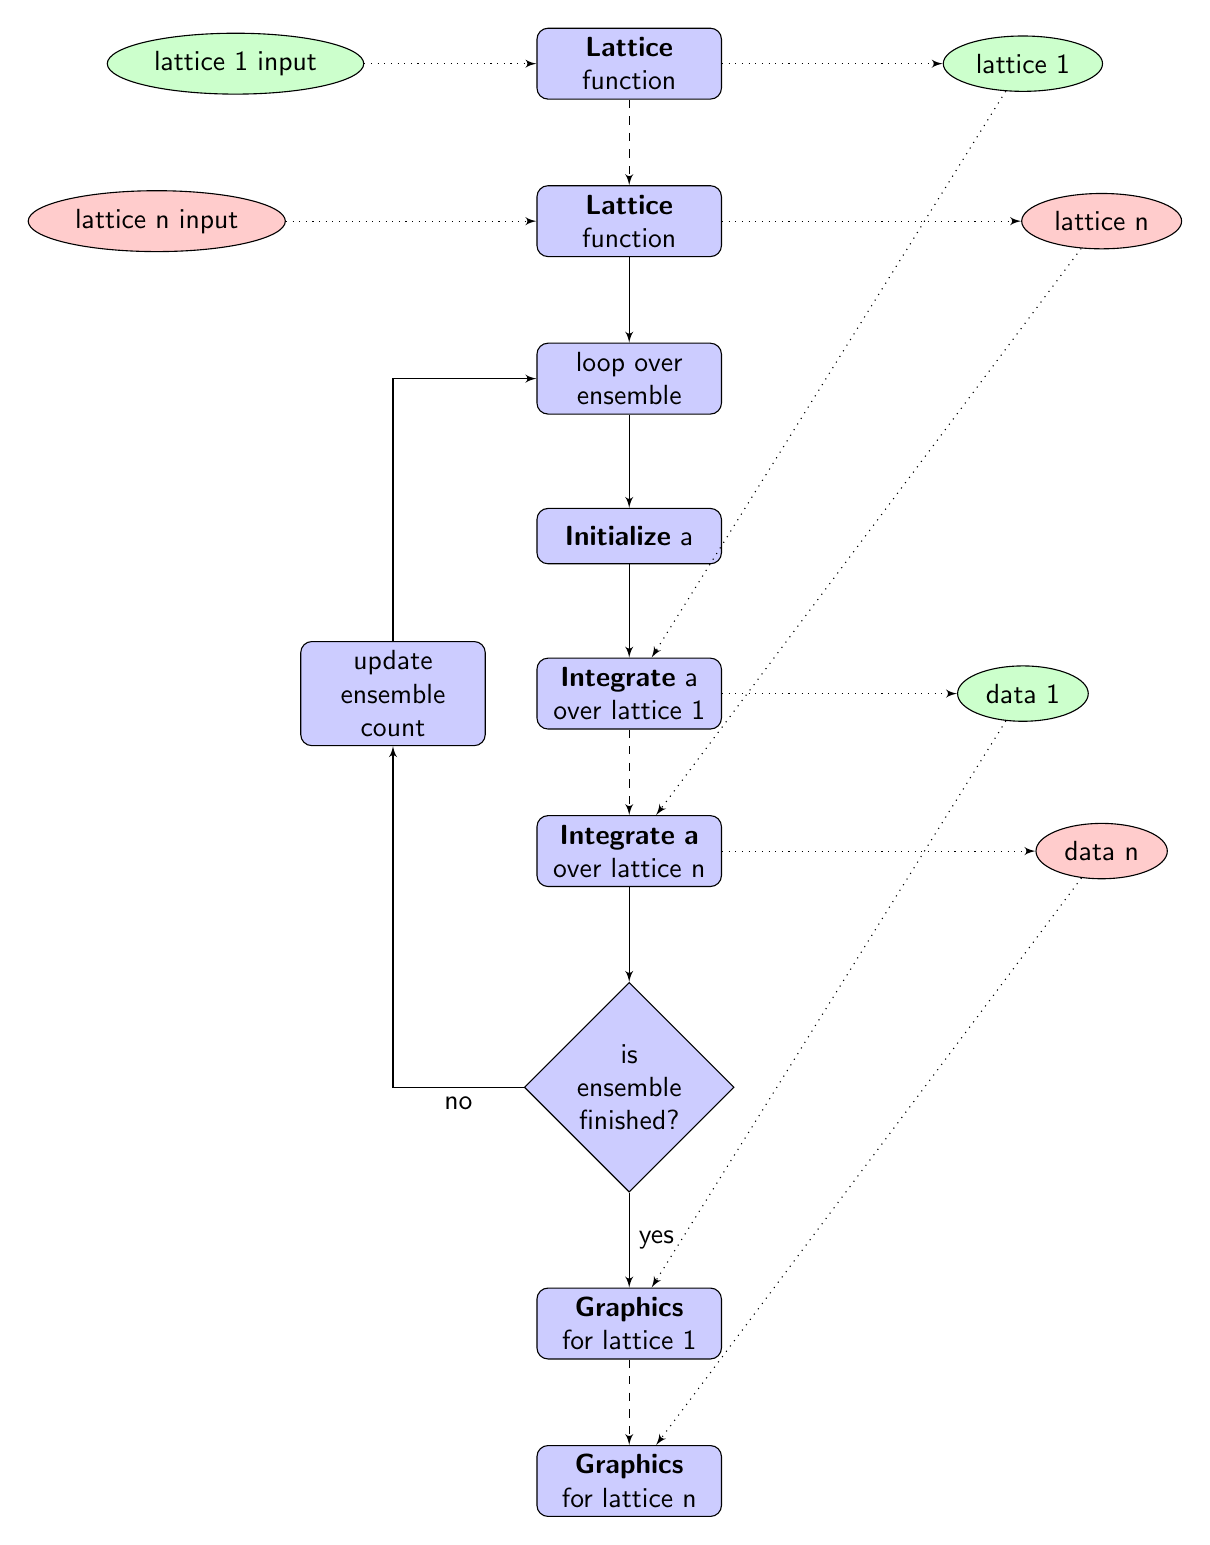
\begin{tikzpicture}[node distance = 2cm, auto]
    % Place nodes
    \node [block] (init1) {{\bf Lattice}  function};
    \node [cloud, left of=init1] (inputs1) {lattice 1 input};
    \node [cloud, right of=init1] (struct1) {lattice 1};

    \node [block, below of=init1] (init2) {{\bf Lattice} function};
    \node [cloud2, left of=init2] (inputs2) {lattice n input};
    \node [cloud2, right of=init2] (struct2) {lattice n };
    \node [block, below of=init2] (loop) {loop over ensemble};
     \node [block, below of=loop] (initialize) {{\bf Initialize} a };
    \node [block, below of=initialize] (integrate1) {{\bf Integrate} a over lattice 1};
     \node [cloud, right of=integrate1] (data1) {data 1};
     \node [block, below of=integrate1] (integrate2) {{\bf Integrate a} over lattice n};
       \node [cloud2, right of=integrate2] (data2) {data n};
    \node [block, left of=integrate1, node distance=3cm] (update) {update ensemble count};
    \node [decision, below of=integrate2] (decide) {is ensemble finished?};
    \node [block, below of=decide, node distance=3cm] (graph1) {{\bf Graphics} for lattice 1};
    \node [block, below of=graph1, node distance=2cm] (graph2) {{\bf Graphics} for lattice n};
    % Draw edges
    \path [line,dashed] (init1) -- (init2);

    \path [line] (init2) -- (loop);
    \path [line] (loop) -- (initialize);
     \path [line] (initialize) -- (integrate1);
    \path [line, dashed] (integrate1) -- (integrate2);
    \path [line] (integrate2) -- (decide);
    \path [line] (decide) -| node [near start] {no} (update);
    \path [line] (update) |- (loop);
    \path [line] (decide) -- node {yes}(graph1);
    \path [line,dashed] (graph1) -- (graph2);
     \path [line,dotted] (integrate1) -- (data1);
       \path [line,dotted] (integrate2) -- (data2);
    \path [line,dotted] (inputs1) -- (init1);
     \path [line,dotted] (inputs2) -- (init2);
    \path [line,dotted] (init1) -- (struct1);
    \path [line,dotted] (init2) -- (struct2);
    \path [line,dotted] (struct1) -- (integrate1);
     \path [line,dotted] (struct2) -- (integrate2);
     \path [line,dotted] (data1) -- (graph1);
     \path [line,dotted] (data2) -- (graph2);


    \end{tikzpicture}

\end{document}
